 \documentclass[11pt, twoside, openany]{book}

%Uncomment the "compresstrue" line and comment out the "compressfalse" line in order to obtain a compressed version of the .pdf file (THIS MIGHT RESULT IN LOW-QUALITY FIGURES!)
\newif\ifcompress
%\compresstrue
\compressfalse

%Uncomment the "printtrue" line and comment out the "printfalse" line to generate a printable PDF (where hyperlinks are not shown with color, but are black)
\newif\ifprint
%\printtrue
\printfalse


% Page setup
 %The following defines an A4 page with classical margin distribution according to the French canon des ateliers: https://tex.stackexchange.com/questions/249190/recommended-margin-and-binding-offset
\usepackage[paperheight=297mm,paperwidth=210mm, bindingoffset=0mm,verbose,marginratio={4:6,5:7},textwidth=140mm,height=213mm,twoside, nomarginpar]{geometry}

% Text and font-related packages
\usepackage[utf8]{inputenc}
\usepackage[german, english]{babel}
\usepackage{newtxtext, newtxmath, cabin}
\usepackage[scaled=0.8]{beramono}
\usepackage[T1]{fontenc}
\usepackage{anyfontsize}

% Math, chemistry, table and figure-related packages
\usepackage{bm}
\usepackage{braket}
\usepackage{dsfont}
\usepackage{etaremune}
\usepackage{graphicx}
\usepackage{mathtools}
\usepackage{microtype}
\usepackage{multicol}
\usepackage{slantsc}
\usepackage[table]{xcolor}
\usepackage{xstring}
\usepackage[version=4]{mhchem}
\usepackage{booktabs}
\usepackage{multirow}
\usepackage{setspace}
\usepackage{lipsum}
\usepackage{enumitem}
\usepackage{pdflscape}
\usepackage{tocbasic}
\usepackage{placeins}

% Table of content style
\DeclareTOCStyleEntry[beforeskip=6pt plus 1pt minus 1pt]{tocline}{chapter}

\makeatletter

% CAPTIONS
\usepackage[font=small, labelfont=bf]{caption, subcaption}

\def\sublabels#1{\foreach \sublabel in {a,b,...,j}
    {\phantomsubcaption\label{#1_\sublabel}}}

% GRAPHICS:
\usepackage{tikz}

\usetikzlibrary{positioning}


% CHAPTER AND SECTION HEADINGS:
\usepackage[immediate]{silence}
\WarningFilter[temp]{latex}{Command} % silence the warning
\usepackage{sectsty}
\DeactivateWarningFilters[temp] % So nothing unrelated gets silenced
\allsectionsfont{\sffamily}

% EPIGRAPHS
\usepackage{epigraph}
\setlength{\epigraphwidth}{0.42\textwidth}
\def\@epitext#1{%
    \begin{minipage}{\epigraphwidth}
        \begin{\textflush}
            \itshape #1
        \end{\textflush}
        \vspace*{1ex}
    \end{minipage}
    }

\def\@episource#1{%
    \begin{minipage}{\epigraphwidth}
        \begin{\sourceflush}
            ---#1
        \end{\sourceflush}
    \end{minipage}
    }

% HEADERS AND FOOTERS
\usepackage{fancyhdr}
\usepackage[breakall, fit]{truncate}

\pagestyle{fancy}

\fancyhf{}

\def\headerline#1{\MakeUppercase{\truncate{0.7\linewidth}{#1}}}

\def\chaptermark#1{\markboth
    {\if@mainmatter\thechapter\quad\fi\headerline{#1}}
    {\headerline{#1}\if@mainmatter\quad\thechapter\fi}}

\def\sectionmark#1{\markright
    {\headerline{#1}\if@mainmatter\quad\thesection\fi}}

\fancyhead[OL]\leftmark
\fancyhead[ER]\rightmark
\fancyhead[OR]\thepage
\fancyhead[EL]\thepage

\setlength\headheight{14pt}
\def\headrulewidth{0.4pt}
\def\footrulewidth{0pt}

% COLORS
\definecolor{linkcolor}{rgb}{0.5, 0.0, 0.0}
\definecolor{basiccolor}{rgb}{0.1, 0.3, 0.5}
\definecolor{commentcolor}{rgb}{0.5, 0.5, 0.5}
\definecolor{identifiercolor}{rgb}{0.2, 0.2, 0.2}
\definecolor{keywordcolor}{rgb}{0.0, 0.4, 0.8}
\definecolor{numbercolor}{rgb}{0.5, 0.5, 0.5}
\definecolor{stringcolor}{rgb}{0.0, 0.4, 0.8}

% SOURCE CODE LISTINGS 
\usepackage{listings}
\lstdefinelanguage{f90}{
    keywords = {
        allocate,
        enddo,
        read,
        external,
        call,
        size,
        if,
        then,
        open,
        write,
        close,
        endif,
        module,
        use,
        only,
        save,
        integer,
        allocatable,
        real,
        logical,
        end,
        complex,
        do,
        cycle,
        character,
        namelist,
        return,
        subroutine,
        intent,
        },
    comment = [l]{!},
    string = [d]',
    morestring = [d]",
    sensitive = false,
    %
    escapeinside = ||,
    moredelim=**[is][\color{red}\underbar]{>>}{<<},
    }

\lstdefinelanguage{py}{
    keywords = {
        and,
        as,
        assert,
        break,
        class,
        continue,
        def,
        del,
        elif,
        else,
        except,
        exec,
        finally,
        for,
        from,
        global,
        if,
        import,
        in,
        is,
        lambda,
        not,
        or,
        pass,
        print,
        raise,
        return,
        try,
        while,
        with,
        yield,
        },
    comment = [l]{\#},
    string = [b]',
    morestring = [s]{r'}{'},
    morestring = [b]",
    morestring = [s]{r"}{"},
    sensitive = true,
    }

\lstdefinelanguage{bash}{
    keywords = {
        in,
        do,
        done,
        for,
        mpirun,
        python3,
        tee,
        test,
        },
    alsoletter = {., -, /, :},
    comment = [l]{\#},
    string = [b]',
    morestring = [b]",
    sensitive = true,
    }

\lstdefinelanguage{qe}{
    comment = [l]{!},
    string = [d]',
    }

\lstset{
    basicstyle = \color{basiccolor} \ttfamily,
    commentstyle = \color{commentcolor},
    identifierstyle = \color{identifiercolor},
    keywordstyle = \color{keywordcolor} \bfseries,
    numberstyle = \color{numbercolor} \scriptsize,
    stringstyle = \color{stringcolor},
    %
    numbers = left,
    showstringspaces = false,
    breaklines = false,
    breakatwhitespace = true,
    showlines = true,
    %
    aboveskip = 3mm,
    belowskip = 3mm,
    numbersep = 3mm,
    }

% Marco Daniel @ https://tex.stackexchange.com/questions/34094/suppress-line-numbering-for-specific-lines-in-listings-package

\def\lstnew{%
    \lst@AddToHook{OnNewLine}{%
    \def\thelstnumber{+}%
    \color{red}%
    \definecolor{commentcolor}{named}{red}%
    \definecolor{identifiercolor}{named}{red}%
    \definecolor{keywordcolor}{named}{red}%
    \definecolor{numbercolor}{named}{red}%
    \definecolor{stringcolor}{named}{red}%
    \advance\c@lstnumber-\@ne}}

\def\lstold{\expandafter\gdef\csname\@lst hk@OnNewLine\endcsname{}}

\newcommand\code[2][bash]{\text{\lstinline[language=#1]{#2}}}

% ACRONYMS:
\usepackage{acronym} % printonlyused, withpage
\usepackage{letltxmacro}
\renewcommand*{\aclabelfont}[1]{\textbf{\boldmath\acsfont{#1}}} %https://tex.stackexchange.com/questions/229930/bolding-math-acronyms


\def\acromod#1{#1}

\foreach \acromacro in {acro,acroplural} {
    \expandafter\xdef\csname\acromacro new\endcsname##1{%
        \noexpand\@ifnextchar[
            {\csname\acromacro newopt\endcsname{##1}}
            {\csname\acromacro newnop\endcsname{##1}}}
    \expandafter\xdef\csname\acromacro newopt\endcsname##1[##2]##3{%
        \csname\acromacro old\endcsname{##1}[##2]{%
            \noexpand\protect\noexpand\acromod ##3}}
    \expandafter\xdef\csname\acromacro newnop\endcsname##1##2{%
        \csname\acromacro old\endcsname{##1}{%
            \noexpand\protect\noexpand\acromod ##2}}
    }

\foreach \acrosuffix in {,f,l,s,p,fp,lp,sp,fi,lu} {
    \edef\acromacro{ac\acrosuffix}
    \edef\Acromacro{Ac\acrosuffix}
    \protected\expandafter\xdef\csname \Acromacro\endcsname{%
        \noexpand\@ifstar
            {\csname @\Acromacro star\endcsname}
            {\csname @\Acromacro nost\endcsname}}
    \expandafter\xdef\csname @\Acromacro star\endcsname##1{%
        {\noexpand\let\noexpand\acromod\noexpand\MakeUppercase%
            \csname \acromacro\endcsname*{##1}}}
    \expandafter\xdef\csname @\Acromacro nost\endcsname##1{%
        {\noexpand\let\noexpand\acromod\noexpand\MakeUppercase%
            \csname \acromacro\endcsname{##1}}}
    }

\def\ainclude#1{\include{#1}\input{#1.uac}}
\def\tinclude#1{\include{#1}\input{#1.uac}}

% DEDICATION page
\newenvironment{dedication}
  {
   \thispagestyle{empty}
   \vspace*{\stretch{1}}
   \itshape             
   \raggedleft
  }
  {\par
   \vspace{\stretch{3}}
   \clearpage          
  }


% BIBLIOGRAPHY: This uses APSREV 4.1 standards, change as needed
\usepackage[numbers, sort&compress]{natbib}
\bibliographystyle{apsrev4-1}

\def\ccite#1{Ref\IfSubStr{#1}{,}{s}{}.~\citenum{#1}}
\def\cfcite#1{\cf{\ccite{#1}}}

% HYPERLINKS (shown in red color if print=true, otherwise they stay black)
\ifprint
\usepackage[pdfa, hidelinks, allcolors=linkcolor, backref=page, pdfencoding=auto]{hyperref}
\else
\usepackage[pdfa, colorlinks, allcolors=linkcolor, backref=page, pdfencoding=auto]{hyperref}
\fi

\def\backref#1{}
\def\backrefalt#1#2#3#4{\ifcase#1 Not cited\or Cited on page~#2\else Cited on pages~#2\fi.}

\backrefparscanfalse
\def\BibitemShut#1{\csname bibitem#1\endcsname\backrefprint}%
\usepackage{hypernat}

% REFERENCES
\usepackage[capitalise]{cleveref}

\crefname{appendix}{App.}{Apps.}
\crefname{chapter}{Chap.}{Chaps.}
\crefname{equation}{Eq.}{Eqs.}
\crefname{figure}{Fig.}{Figs.}
\crefname{section}{Sec.}{Secs.}
\crefname{table}{Tab.}{Tabs.}
\Crefname{appendix}{Appendix}{Appendices}
\Crefname{chapter}{Chapter}{Chapters}
\Crefname{equation}{Equation}{Equations}
\Crefname{figure}{Figure}{Figures}
\Crefname{section}{Section}{Sections}
\Crefname{table}{Table}{Tables}

\creflabelformat{equation}{#2\textup{#1}#3}

\def\creflastconjunction{, and~}

\makeatother
\def\see#1{(#1)}
\def\cf#1{\see{cf.\@ #1}}
\def\cfref#1{\cf{\cref{#1}}}
\def\seeref#1{\see{\cref{#1}}}
\makeatletter

% Heiko Oberdiek @ https://tex.stackexchange.com/questions/340492/can-cref-be-made-to-ignore-spaces
\let\org@@cref\@cref
\renewcommand*{\@cref}[2]{%
  \begingroup
    \toks@={}%
    \comma@parse{#2}\add@cref@item
  \edef\process@me{\endgroup
    \noexpand\org@@cref{#1}{\the\toks@}%
  }\process@me
}
\newcommand*{\add@cref@item}[1]{%
  \expandafter\ifx\expandafter\\\the\toks@\\%
    \toks@{#1}%
  \else
    \toks@\expandafter{\the\toks@,#1}%
  \fi
}

\makeatother

% TABLE OF CONTENTS
\setcounter{tocdepth}{3} %This defines up to which depth the Table of contents is printed, e.g. Sec. 3.2.1.5.3 would be tocdepth 5, Sec. 1.2 would be tocdepth 2
\setcounter{secnumdepth}{3}

% FLOATS
\setcounter{topnumber}{1}
\setcounter{bottomnumber}{1}

% This prevents LATEX from cramping text between two figures when they are close
\def\textfraction{0.1}
\def\topfraction{0.9}
\def\bottomfraction{0.9}
\def\floatpagefraction{0.9}

\onehalfspacing %This sets the spacing between your lines, change for \doublespacing for larger distances

% PENALTIES: This avoids widows and orphans (https://en.wikipedia.org/wiki/Widows_and_orphans)
\clubpenalty=10000
\widowpenalty=10000
\displaywidowpenalty=10000
\interfootnotelinepenalty=10000


%This defines a few useful macros
\def\centered#1#2{\hspace{0pt}\llap{#1}\hspace{1pc}\rlap{#2}}

\def\todo#1{\textcolor{red}{#1}}

\def\nonumsection#1{
    \phantomsection
    \addcontentsline{toc}{section}{#1}
    \section*{#1}
    }

%This defines the appearence of the "remarks" blocks that can be placed in the beginning of every chapter
\newenvironment{remarks}
{%
    \begin{equation*}
        \color{black!90}
        \hspace*{-1cm}
        \left[
        \hspace{1mm}
        \begin{minipage}{\linewidth} \itshape
}{%
        \end{minipage}
        \hspace{1mm}
        \right]
        \hspace*{-1cm}
    \end{equation*}
}

\def\remark#1{\emph{\color{black!90}[#1]}}

\newenvironment{codecols}[1][\relax]
{%
    \begingroup
        #1
        \vspace*{-1mm}
        \begin{multicols}{2}
}{%
        \vspace*{-3mm}
        \end{multicols}
    \vspace*{-3mm}
    \endgroup
    \noindent
    \ignorespacesafterend
}


% Herbert/user2478 @ https://tex.stackexchange.com/questions/10141/how-to-prevent-lstlisting-from-splitting-code-between-pages
\lstnewenvironment{nobrlstlisting}[1][]%
  {\endgraf\noindent\minipage{\linewidth}\lstset{#1}}
  {\endminipage\endgraf}

% This devines the appearance of many mathematical/physical symbols and operators
\let\temporary\epsilon
\let\epsilon\varepsilon
\let\varepsilon\temporary
\let\temporary\phi
\let\phi\varphi
\let\varphi\temporary
\let\temporary\Pi
\let\Pi\varPi
\let\varPi\temporary
\let\temporary\Theta
\let\Theta\varTheta
\let\varTheta\temporary
\let\mat\relax
\let\op\hat
\let\tilde\widetilde
\let\vec\bm
\let\x\times
\let\X\texttimes
\let\up\uparrow
\let\down\downarrow
\let\pit\pi
\let\pi\uppi
\let\Re\relax
\let\Im\relax

\DeclareMathOperator\Re{Re}
\DeclareMathOperator\Im{Im}
\DeclareMathOperator\diag{diag}
\DeclareMathOperator\erf{erf}
\DeclareMathOperator\erfc{erfc}

\def\D{\mathrm d}
\def\E{\mathrm e}
\def\I{\mathrm i}
\def\K{\mathrm K}
\def\M{\mathrm M}
\def\g{\color{gray}}
\def\n{\phantom0}
\def\p{\phantom+}

\def\Vec#1{\underline{\vec{#1}}}
\def\sub#1{\sb{\textnormal{#1}}}
\def\super#1{\sp{\textnormal{#1}}}
\def\from#1{\sb{\mathrlap{#1}}}
\def\till#1{\sp{\mathrlap{#1}}}
\def\limit#1{\sp{\mathclap{#1}}}
\def\bra#1{\langle#1|}
\def\ket#1{|#1\rangle}
\def\bracket#1#2{\langle#1|#2\rangle}
\def\av#1{\langle#1\rangle}
\def\abs#1{|#1|}
\def\adj{^\dagger}
\def\padj{^{\vphantom\dagger}}
\def\conj{^\ast}
\def\pconj{^{\vphantom\ast}}
\def\trans{^{\mathrm T}}
\def\ptrans{^{\mathrm T}}
\def\inv{^{-1}}
\def\pinv{^{\vphantom{-1}}}
\def\pprime{^{\vphantom\prime}}
\def\tilded{\tilde{\vphantom{t}\smash[t]{d}}}
\def\notsubseteq{\expandafter\not\protect\subseteq}

% Insert your own commonly used abbreviations (such as chemical formulae) here!
\def\NbSeII{NbSe\texorpdfstring{\s2}{\texttwoinferior}}
\def\QE{\textsc{Quantum ESPRESSO}\,}

\def\placeholder{\mathord{\color{gray}\bullet}}

% Collections of references:
% EXAMPLE
\newcommand{\hubbard}{\cite{hubbardElectron1963,hubbardElectron1964,hubbardElectron1964a}}



\def\includeonly#1{}


%This list defines the order in which the .tex files are included to compose the final document.
%Add or remove sections as needed
%
\begin{document}
    \frontmatter
    \ifprint\else
\newgeometry{margin=3cm}
\fi

\begin{titlepage}
    \centering

    \normalsize
    \includegraphics[height=1.5cm]{I_figures/UNILOGO.pdf}\hfill
    
\includegraphics[height=1.5cm]{I_figures/HMI.png}\\

% Adjust this text according to the faculty's requirements! Note that the text changes once the thesis is approved and you have to hand in a copy to the library!

    \vfill

    \large
    Dem Fachbereich Produktionstechnik der \\
     \vspace{1em}
     
    UNIVERSITÄT BREMEN \\
     \vspace{1em}
     
    zur Erlangung des Grades \\
     \vspace{1em}
     
    Doktor der Ingenieurwissenschaften (Dr.-Ing.) \\
    \vspace{1em}
    
    vorgelegte Dissertation


    \vspace{3pc}

% Titles in English and German
    \Huge \sffamily
    \textbf{My PhD thesis title}

    \vspace{3pc}

    \normalsize \normalfont
    \textit{Der Titel meiner Doktorarbeit}

    \vfill
    \large

% Author information and supervisor information
    \centered{von}{John Doe, M. Sc.}

    \vspace{1pc}

    \centered{geboren am}{01. Januar 1990}

    \vspace{1pc}
        
    \centered{in}{Springfield, USA}

    \vspace{3pc}

    \centered{Erstgutachter}{Prof.\@ Dr.\@ Lucio Colombi Ciacchi}\\
    \centered{Zweitgutachter}{Prof.\@ Dr.\@ Stephen Hawking (University of Cambridge)}

    \vspace{3pc}

%Date of hand-in
    Eingereicht am 01.\@ Januar 3000

    \vfill
\end{titlepage}

\ifprint\else
\restoregeometry
\fi

\thispagestyle{plain}

\vspace*\fill

\bigskip

% Copyright statements of already published works. Adapt according to the editorial's requirements!
\noindent
Parts of \cref{cha:first-results} reprinted with permission from J. Chem.\@ Theory \@  Comput.~\textbf{20}, 11, 4824-4843 \textcopyright{} 2024 American Chemical Society.\\
Parts of \cref{cha:second-results}  reprinted with permission from J. Chem.\@ Theory \@  Comput.~\textbf{22}, 2, 1016-1029 \textcopyright{} 2026 American Chemical Society.
\bigskip


\noindent
Typeset with {\LaTeX} in New TX, \textsf{Cabin}, and \texttt{Bera Mono}.

\bigskip

\noindent

    \begin{dedication}
    Dedicated to whoever you like.
\end{dedication}



    \chapter*{Abstract}
\singlespacing %Abstract should not have large linespacing
    %
    \Ac{DFT} Lorem ipsum dolor sit amet, consetetur sadipscing elitr, sed diam nonumy eirmod tempor invidunt ut labore et dolore magna aliquyam erat, sed diam voluptua.
    %
    At vero eos et accusam et justo duo dolores et ea rebum.
    %
    Stet clita kasd gubergren, no sea takimata sanctus est Lorem ipsum dolor sit amet.
    %
    Lorem ipsum dolor sit amet, consetetur sadipscing elitr, sed diam nonumy eirmod tempor invidunt ut labore et dolore magna aliquyam erat, sed diam voluptua.
    %
    At vero eos et accusam et justo duo dolores et ea rebum.
    %
    Stet clita kasd gubergren, no sea takimata sanctus est Lorem ipsum dolor sit amet. \medskip
    %
    
    \noindent  Lorem ipsum dolor sit amet, consetetur sadipscing elitr, sed diam nonumy eirmod tempor invidunt ut labore et dolore magna aliquyam erat, sed diam voluptua.
    %
    At vero eos et accusam et justo duo dolores et ea rebum.
    %
    Stet clita kasd gubergren, no sea takimata sanctus est Lorem ipsum dolor sit amet.
    %
    Lorem ipsum dolor sit amet, consetetur sadipscing elitr, sed diam nonumy eirmod tempor invidunt ut labore et dolore magna aliquyam erat, sed diam voluptua.
    %
    At vero eos et accusam et justo duo dolores et ea rebum.
    %
    Stet clita kasd gubergren, no sea takimata sanctus est Lorem ipsum dolor sit amet. \medskip
    %
    


%%%%%%%%%%%%%%%%%%%%%%%%%%%%%%%%%%%%%%%%%%%%%%%%%%%%%%%%%
\begingroup
\selectlanguage{german}

\chapter*{Kurzzusammenfassung}
    \Ac{DFT} Lorem ipsum dolor sit amet, consetetur sadipscing elitr, sed diam nonumy eirmod tempor invidunt ut labore et dolore magna aliquyam erat, sed diam voluptua.
    %
    At vero eos et accusam et justo duo dolores et ea rebum.
    %
    Stet clita kasd gubergren, no sea takimata sanctus est Lorem ipsum dolor sit amet.
    %
    Lorem ipsum dolor sit amet, consetetur sadipscing elitr, sed diam nonumy eirmod tempor invidunt ut labore et dolore magna aliquyam erat, sed diam voluptua.
    %
    At vero eos et accusam et justo duo dolores et ea rebum.
    %
    Stet clita kasd gubergren, no sea takimata sanctus est Lorem ipsum dolor sit amet. \medskip
    %
    
    \noindent  Lorem ipsum dolor sit amet, consetetur sadipscing elitr, sed diam nonumy eirmod tempor invidunt ut labore et dolore magna aliquyam erat, sed diam voluptua.
    %
    At vero eos et accusam et justo duo dolores et ea rebum.
    %
    Stet clita kasd gubergren, no sea takimata sanctus est Lorem ipsum dolor sit amet.
    %
    Lorem ipsum dolor sit amet, consetetur sadipscing elitr, sed diam nonumy eirmod tempor invidunt ut labore et dolore magna aliquyam erat, sed diam voluptua.
    %
    At vero eos et accusam et justo duo dolores et ea rebum.
    %
    Stet clita kasd gubergren, no sea takimata sanctus est Lorem ipsum dolor sit amet. \medskip

\endgroup

\vspace*{-10cm}


\onehalfspacing
    \chapter*{Contents}

\makeatletter
\@starttoc{toc}
\makeatother

    \chapter{List of Figures}

\makeatletter
\@starttoc{lof}
\makeatother

\section*{Tables}

\makeatletter
\@starttoc{lot}
\makeatother

    \chapter{List of Acronyms}

\begingroup
\makeatletter
\def\AC@hyperref[#1]#2{#2}
\makeatother
\begin{acronym}
    \LetLtxMacro\acroold\acro
    \LetLtxMacro\acro\acronew
    \LetLtxMacro\acropluralold\acroplural
    \LetLtxMacro\acroplural\acropluralnew
    %
    \acro{BO}{Born--Oppenheimer\acroextra{ (approximation)~\cite{bornZur1927}}}
    \acro{BZ}{Brillouin zone}
    \acro{CT}{charge-transfer\acroextra{ (insulator)}}
    \acro{DC}{double counting\acroextra{ (term)}}
    \acro{DFT}{density-functional theory}
    \acro{FCC}{face-centered cubic\acroextra{ (Bravais lattice)}}
    \acro{GPU}{graphics processing unit}
    \acro{HOMO}{highest occupied molecular orbital}
    \acro{KS}{Kohn--Sham}
    \acro{LDA}{local-density approximation}
    \acro{LUMO}{lowest unoccupied molecular orbital}
    \acro{MAE}{mean average error}
    \acro{ML}{machine-learning}
    \acro{MO}{molecular orbital}
    \acro{PDOS}{projected density of states}
    \acro{PES}{potential energy surface}
    \acro{QE}{\textsc{Quantum ESPRESSO}\acroextra{ (software suite)~\cite{giannozziQUANTUM2009,giannozziAdvanced2017,giannozziQuantum2020}}}
    \acro{SOC}{state of charge\acroextra{ (of a battery)}}
    \acro{xc}{exchange--correlation\acroextra{ (functional)}}

    % Define atypical plural forms here:
    \acroplural{DOS}[DOS]{densities of states}
    \acroplural{SOC}[SOC]{states of charge}
\end{acronym}
\endgroup

    \chapter{List of Symbols}
%These are just examples; define symbols according to your needs.
\singlespacing
\begin{multicols}{2}
\begin{description}
    \item[$E$] total energy
    \item[$H$] Hamiltonian
    \item[$\sigma$, $\uparrow, \downarrow$] spin indices of electronic orbitals
    \item[$\psi$] electronic or Kohn--Sham wave function
    \item[$\Psi$] many-body wave function
    \item[$\varphi$] (orthogonalized) atomic orbital
    \item[$\phi$] diagonal projector orbital
    \item[$\mathbf{n}$] (projected) occupation matrix
    \item[$\lambda$] eigenvalue (of the occupation matrix)
    \item[$\nu$] eigenvector (of the occupation matrix)
    \item[$i, j$] indices of eigenstates or orbitals
    \item[$I, J$] indices of atoms
    \item[$v$] index of electronic bands
    \item[$x, y, z$] indices of Cartesian directions
    \item[$M$] atomic mass
    \item[$J$] unlike-spin Hund parameter
    \item[$U$] on-site Hubbard parameter
    \item[$V$] inter-site Hubbard parameter
    \item[$W$] fully screened Coulomb interaction
    \item[$f$] Fermi function
    \item[$T$] temperature
    \item[$\chi_0$] bare electronic response
    \item[$\chi$]   screened electronic response
    \item[$\vec a, \vec b, \vec c$] Bravais basis vectors
    \item[$\vec R$] nuclear position
    \item[$\vec r$] fermionic position in real space
    \item[$\vec k$] fermionic wave vector
    \item[$\vec q$] bosonic wave vector %TODO: fix
    \item[$\vec F$] Force vector
    \item[$N$] number of lattice points
    \item[$\placeholder \conj$] complex conjugate
    \item[$m \sub e = 1$] electron mass
    \item[$e = 1$] elementary charge
    \item[$\hbar = 1$] reduced Planck constant
    \item[$k \sub B = 1$] Boltzmann constant
    \item[$1 / 4 \pi \varepsilon_0 = 1$] Coulomb constant
\end{description}
\end{multicols}
    \mainmatter
    \chapter[Template introduction]{How to use the HMI thesis template in practice} % The title in square brackets is the one printed in the Table of contents, and should thus be reasoanbly short
    \label{cha:introduction}
    %
    \onehalfspacing
    %
\epigraph{%.
    The real voyage of discovery consists not in seeking new landscapes, but in having new eyes.}
    {Marcel Proust}
    %
    \begin{enumerate}
        \item In definitions.tex, (re)define the mathematical operators and symbols that you use frequently. Also define other very common abbreviations that you'll need several times, such as chemical formulae, collections of references, etc. 
        %
        \item In packages.tex, define the page geometry with the margins and eventual printing offsets (the default uses the very asthetic french canon des ateliers aspect ratios with 1/3 of the page as margins). Then load any additional \LaTeX packages that you might need.
        %
        \item Review the values in settings.tex, mainly tocdepth and spacing (single, onehalf, double).
        %
        \item In acronyms.tex, define your acronyms paying attention to the use of plural forms. Read up on how to use the acronyms package: \url{https://www.namsu.de/Extra/pakete/Acronym.html}
        %
        \item Define all important mathematical/physical symbols in symbols.tex
        %
        \item Adjust the title page in titlepage.tex. Fulfill all requirements of the faculty to which you submit! Also, provide adequate copyright statements if you are using already published works for your thesis chapters. Always review the requirements of the publishers (ACS, APS, RSC, etc.).
        %
        \item Now, you can start renaming and reordering the chapters defined in IV\_mainmatter using the thesis.tex file, and finally start to work on your thesis!
    \end{enumerate}

    \textbf{General tips for thesis writing and the use of \LaTeX}
    %
    \begin{itemize}
        \item If you recompile the document and get new errors and/or warnings, \textbf{ALWAYS FIX THEM IMMEDIATELY}. Do not let errors accumulate, as it might get close to impossible to debug them once they pile up and start to interact. You will run into compile timeouts if you have a large document with tons of Latex errors.
        %
        \item Do not cramp too much text into one line. This makes debugging very hard, as Latex will only show you "Error in line X", but if line X contains 1000 words, good luck spotting the issue.
        %
        \item Instead, write only one sentence per line. You can even separate two sentences by a \% sign for better visuals
        %
        \item Use indentation to improve the visual clarity
        %
        \item Always label your chapters, sections, figures and tables immediately and in a systematic and understandable way. This will make it a lot easier to use the ref command when you want to refer to the object
        %
        \item Use multiple .tex files for long documents like PhD theses and "glue" them together through the thesis.tex file using the include command. If you put 100000 words in a single .tex file, you'll take forever to find any text that you might need to change
        %
        \item When creating figures, try to use vector formats (.svg, .eps, .pdf in some cases) over raster formats whenever possible. Create your figures exactly according to the page dimensions defined in packages.tex (e.g., a width of 140mm if textwidth=140mm). Alternatively, for many graphs you can also use the tickz package
        %
        \item Read up on the basic rules of good typesetting before you begin. For example, between a value and its corresponding unit, there should be a half space, i.e: The temperature was 500\,K rather than 500 K or 500K. Remember that units and chemical symbols should never be italicized. Also know which kind of dash to use: hyphens (-) for connected words like well-known, En dashes (--) for ranges like 20--30\,mg, and Em dashes (---) for breaking sentences: Birds---such as pigeons---are animals that have wings.
    \end{itemize}
    \chapter[Figures, Tables, References]{Figures, Tables, and References}
    \label{cha:figures}

\epigraph{%
    The underlying physical laws necessary for the mathematical theory of a large part of physics and the whole of chemistry are thus completely known, and the difficulty is only that the exact application of these laws leads to equations much too complicated to be soluble.}
    {P.~A.~M.~Dirac}

% The following space can be used as a "section abstract" where you summarize the work and its main findings.
%
\noindent This chapter explains the use figures, tables, references and other things important to a PhD thesis typeset with \LaTeX.
%%%%%%%%%%%%%%%%%%%%%%%%%%%%%%%%%%%%%%%%%%%%%%%%%%%%%%%%%%%%%%%%%%%%
% The main content of the chapter begins here
%
\section{Including and referencing figures}
    \label{sec:figures}
    %
    \subsection{A first figure}
        \label{subsec:figures1}
    %
    \Cref{fig:02-PWL} shows how to include a figure.
    %
    Make sure that you understand the float modifiers of the figure environment (i.e., the letters t, b, h, p, and the exclamation mark)
    %
    Always provide a short caption in square brackets, as the long caption is often way too long for the List of Figures.
    %
    Label your figures clearly and systematically, as this will make your life easier once you begin referring to your figures \seeref{subsec:references} .
    %
    \begin{figure}[t]
    \centering
        \includegraphics[width=1.0\textwidth]{I_figures/02_1_PWL.png}
        \caption[Short caption of the PWL condition figure.]{Schematic illustration of the ground-state total energy as a function of electron number. The exact energy is PWL between integer occupations, whereas (semi)local \ac{xc} functionals exhibit a spurious convex curvature. Small misalignments at integer $n$ indicate residual ``endpoint'' errors, as approximate \ac{DFT} is not exact even for integer electron numbers.}
        \label{fig:02-PWL}
    \end{figure}
    %
%%%%%%%%%%%%%%%%%%%%%%%%%%%%%%%%%%%%%%%%%%%%%%%%%%%%%%%%%%%%%%%%%%%%
    \subsection{Another section, another figure}
        \label{subsec:figures2}
    %
    \Cref{fig:02-uimpact} shows another example of a figure; namely one that is scaled down to 90\% of  textwidth.
    %
    Note that the imagefiles are named in a systematic manner (02 for chapter 02=theory and \_2 as it is the second figure shown in this chapter).
    %
    This helps to avoid confusion at later stages of your work, when you have dozens of imagefiles with potentially similar names.
    %
    \begin{figure}[ht]
    \centering
        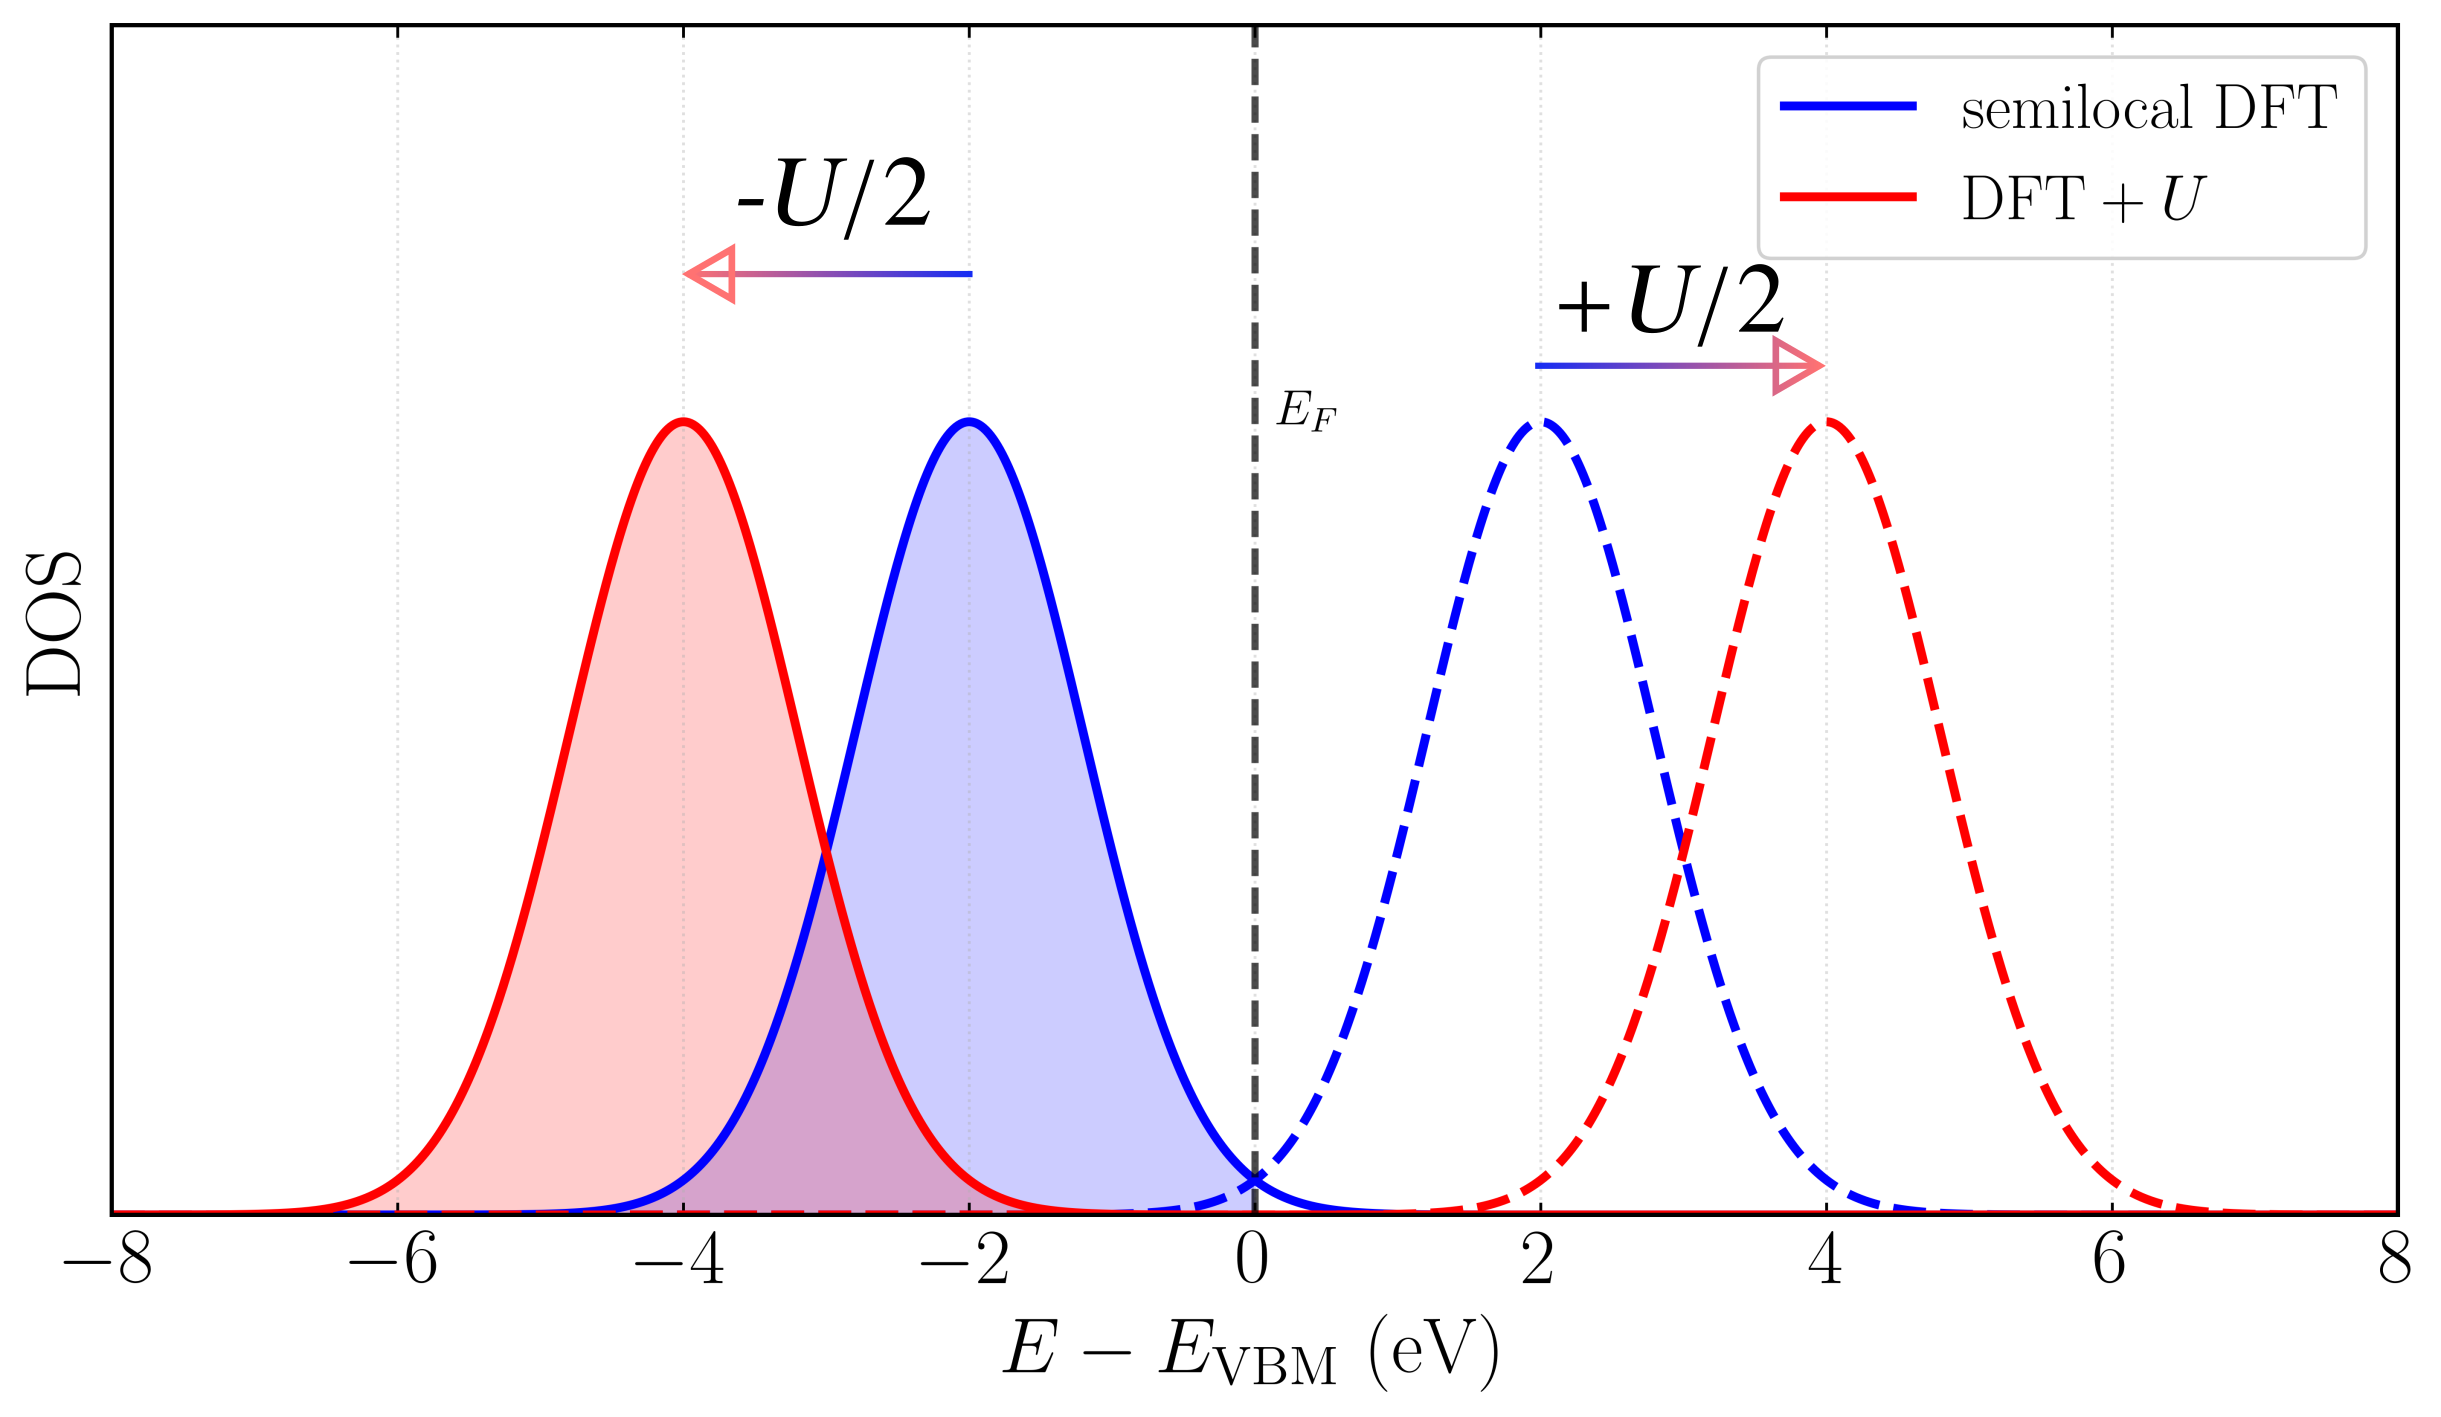
\includegraphics[width=0.9\textwidth]{I_figures/02_2_U-Impact.png}
        \caption[Potential shift due to Hubbard $U$ corrections.]{Impact of an on-site $U$ correction (Dudarev functional) on the energetic levels of the occupied (solid lines) and unoccupied (dashed lines) states of an isolated manifold. The potential of the states is shifted by $\pm U/2$ (here: $U\approx4\,$eV), thus leading to the emergence of a band gap.}
        \label{fig:02-uimpact}
    \end{figure}
    %
%%%%%%%%%%%%%%%%%%%%%%%%%%%%%%%%%%%%%%%%%%%%%%%%%%%%%%%%%%%%%%%%%%%%
\section{Other important things you should know}
      \label{sec:fundamentals}
    %
    \subsection{Internal references}
        \label{subsec:references}
    %
    To refer to chapters, sections, figures, tables, and equations, use the cref command (e.g., \cref{fig:02-PWL}), thanks to which you don't need to put a tilde between the dot after "Fig."., which is required in case you use the classical "ref" command: Fig.~\ref{fig:02-PWL}.
    %
    You can also refer to multiple objects in one command, e.g., \cref{cha:second-results,cha:conclusions}.
    %
    Thanks to the the seeref and cfref macros, \LaTeX automatically renders paraenthesis and puts a "see" or "cf." in front of the reference:  \seeref{cha:conclusions}, \cfref{tab:02-parameters}.
    %
    Make sure you understand the difference between "see" and "cf."!
    %
%%%%%%%%%%%%%%%%%%%%%%%%%%%%%%%%%%%%%%%%%%%%%%%%%%%%%%%%%%%%%%%%%%%%
    \subsection{Citations}
        \label{subsec:citations}
    %
    You have plenty of options to cite works using the natbib package.
    %
    Besides the traditional cite command \cite{andersonMore1972}, you can also make latex print the author's name \textit{together with the citation} (\citet{andersonMore1972}), or without it: \citeauthor{andersonMore1972}.
    %
    Of course, you can also cite multiple references at once: \cite{bornZur1927,giannozziQUANTUM2009,giannozziQuantum2020}.
    %
    If youu want to explicitly refer to a reference, you can print the reference number without the brackets using citenum, e.g., Ref.~\citenum{andersonMore1972}.

    In any case, you should use a consistent naming scheme for your references \textit{from the beginning}, e.g FirstauthornameShorttitleYear.
    %
    Moreover, make sure to avoid unicode symbols incompatible with BibTex (such as the long dash).
    %
    A good and free literature management program is Zotero, which is particularly powerful if you install the (also free) BetterBibTex extension.
    %
%%%%%%%%%%%%%%%%%%%%%%%%%%%%%%%%%%%%%%%%%%%%%%%%%%%%%%%%%%%%%%%%%%%%
    \subsection{Acronyms}
        \label{subsec:acronyms}
    %
    The acronyms package can be very helpful both for you and for the reader to avoid confusion over the use of acronyms.
    %
    Once defined in acronyms.tex, you can invoke an acronym using the ac command: \ac{MAE}.
    %
    Note that when an acronym is invoked for the first time, the package will automatically print the long form and the acronym in parenthesis.
    %
    The second time you refer to the same acronym, like \ac{MAE}, only the short form is shown.

    For plural forms, you can use the acp command, which add an "s" to the last word, unless you defined a different plural form: \acp{MAE}.
    %
    If you want to avoid the long version to be shown, you can tell acronyms that the definitions has already been given through acused.
    %
    \acused{GPU}
    %
    Then, when you invoke the acronym, it will not print the long form: \ac{GPU}.
    %
    However, you can enforce the long form (without the short form) through acl---\acl{GPU}---and vice versa, you can enforce the short form using acs: \acs{GPU}.
    %
%%%%%%%%%%%%%%%%%%%%%%%%%%%%%%%%%%%%%%%%%%%%%%%%%%%%%%%%%%%%%%%%%%%%
    \subsection{Tables}
        \label{subsec:tables}
    %
    \Cref{tab:02-parameters} shows an example of a table environment.
    %
    Always remember that tables have titles (above them) rather than captions (below the object).
    %
    A good tool for creating tables in Latex (e.g., with the good-looking booktabs style) can be found at \url{https://tablesgenerator.com/}.
    %
    \begin{table}[ht]
        \centering
        \setlength{\tabcolsep}{4pt}
        \renewcommand{\arraystretch}{1.6} 
        \caption[Short caption of the \ce{AUO4} Hubbard U table.]{Self-consistent Hubbard $U$ parameters obtained from LR-cDFT for three setups (one shell-averaged plus two orbital-resolved) with differently defined Hubbard manifolds. The values in parentheses are those derived and applied by \citet{wardaGetting2025}.}
        %
        \begin{tabular}{c c c c c}
            \arrayrulecolor{black}\hline
              System & \multicolumn{4}{c}{$U$ (eV)} \\  \hline
            \rowcolor{gray!10}[6pt] Shell-averaged
               & A-$3d$ & U-$5f$ & O1-$2p$ & O2-$2p$ \\ 
        
               \ce{\beta-NiUO4} & 7.03 (6.6) & 3.65 (2.6) & 7.56 & 7.97 \\ 
               \ce{MnUO4} & 7.34 (4.4) & 3.92 (2.7) & 7.45 & 7.82 \\ 
               \ce{CoUO4} & 6.19 (5.2) & 3.77 (2.7) & 7.54 & 7.94\\ 
        
            \rowcolor{gray!10}[6pt] Setup (1)
               & A-$3d$ & U-${5f}_{\nu_1-\nu_4}$ & O1-$2p$ & O2-$2p$ \\ 
        
               \ce{\beta-NiUO4} & 7.03 & 1.37 & 7.59 & 7.97 \\ 
               \ce{MnUO4} & 7.17 & 1.38 & 7.49 & 7.87 \\ 
               \ce{CoUO4} & 6.20 & 1.36 & 7.56 & 7.94\\ 
               
            \rowcolor{gray!10}[6pt] Setup (2)
               & A-${\widetilde{t_{2g}}}$ & U-${5f}_{\nu_1-\nu_4}$ & O1-$2p$ & O2-$2p$ \\ 
               
               \ce{\beta-NiUO4} & 7.40 & 1.33 & 7.50 & 7.78 \\ 
               \ce{MnUO4} & 1.27 & 0.93 & 7.40 & 7.74 \\ 
               \ce{CoUO4} & 2.33 & 1.22 & 7.47 & 7.77 \\ 
            \arrayrulecolor{black}\hline       
        \end{tabular}
        \label{tab:02-parameters}
    \end{table}
    %
%%%%%%%%%%%%%%%%%%%%%%%%%%%%%%%%%%%%%%%%%%%%%%%%%%%%%%%%%%%%%%%%%%%%
    \subsection{Equations}
        \label{subsec:eqs}
    %
    Finally, you can typeset equations using the "equation", "gathered" and "align" environments:
    %
    \begin{equation}
     \frac{\partial}{\partial\vec{R}^K}\left\langle \phi^I_m | \psi^\sigma_{\vec{k}v} \right\rangle   \,.
     \label{eq:2-hub-force}
    \end{equation}
    %
    Never forget that equations should also follow punctuation rules, thus ending either with a full stop or with a comma, like in
    \begin{equation}
        \begin{gathered}
        \frac{\partial E_\mathrm{Hub}}{\partial \vec{R}^K} = \sum_{I}\sum_{\sigma,m,m'} \frac{\partial E_\mathrm{Hub}}{\partial n^{I\sigma}_{mm'}} \frac{\partial n^{I\sigma}_{mm'}}{\partial\vec{R}^K} \\
        = \sum_{I}\sum_{\sigma,m,m'} U^I\left( \frac{\delta_{mm'}}{2}-  n^{I\sigma}_{mm'} \right) \frac{\partial n^{I\sigma}_{m'm}}{\partial\vec{R}^K} \, ,
        \end{gathered}
        \label{eq:2-hub-force2}
    \end{equation}
    %
    which represents a complicated force term.
    %
    Again, use a reasonable labeling scheme so that you can easily refer to your equation, e.g. \cref{eq:2-hub-force}, later on.
    \chapter[My first results chapter]{Long version of my first results chapter title}
    \label{cha:first-results}

\epigraph{%
    The way to get good ideas is to get lots of ideas, and throw the bad ones away.}
    {Linus Carl Pauling}

\begin{remarks}
        Here you can explain meta-information on the origin of this chapter: how was the idea underlying this chapter conceived? Who was involved in the work?
        %
        Has this chapter already published? If so, where (use the cite command!)
        %
        Which parts of the manuscript did you prepare, which parts were written by your collaborators?
        %
        Did you create all of the figures by yourself?
\end{remarks}

% The following space can be used as a "section abstract" where you summarize the work and its main findings (here some parts left as an example)
%
\noindent Example text: Having established the foundations of the Hubbard model and its application as a (self-interaction) correction to \ac{DFT}, we now come to the main outcome of this thesis. 
%
In \cref{cha:figures}, we have seen that Hubbard corrections can markedly improve upon the otherwise poor description by many xc-functionals of strongly localized electrons.
%
Now, we show first results.
%%%%%%%%%%%%%%%%%%%%%%%%%%%%%%%%%%%%%%%%%%%%%%%%%%%%%%%%%%%%%%%%%%%%

\section{Some overview}
    \label{sec:first-overview}

\section{Methodology}
    \label{sec:first-methodology}
    %
    \subsection{Some details}
        \label{subsec:first-details}
    %
    \subsection{Other aspects}
        \label{subsec:first-aspects}

\section{My brilliant idea}
    \label{sec:first-idea}
    \chapter[My second results chapter]{Long version of my second results chapter title}
    \label{cha:second-results}

\epigraph{%
    Dans la vie, rien n'est à craindre,\\ tout est à comprendre.\footnotemark}
    {Marie Skłodowska-Curie}

\footnotetext{\emph{%
    Nothing in life is to be feared, it is only to be understood.}}

% Remarks left here as an example
\begin{remarks}
    Example remarks: Barring minor adaptations, this chapter has been submitted to \textsc{arXiv} as is~\ccite{wardaGetting2025} and is currently under review for publication in the \textit{Journal of Chemical Theory and Computation}.
    %
    Kinga Warda carried out the majority of the \ac{DFT} calculations, while I provided guidance on the choice of the Hubbard manifold, performed the symmetry analysis of the eigenstates, and ran the HSE06 calculations. 
    %
    I also identified the spurious Hubbard force contributions described in \cref{sec:second-spurious}, created three figures (using a plotting utility developed by Iurii Timrov), and authored the majority of the manuscript. 
    %
    Iurii Timrov, Lucio Colombi Ciacchi and Piotr Kowalski supervised the project and assisted in the preparation of the manuscript.
\end{remarks}

% The following space can be used as a "section abstract" where you summarize the work and its main findings (here some parts left as an example)
%
\noindent \Ac{DFT} Lorem ipsum dolor sit amet, consetetur sadipscing elitr, sed diam nonumy eirmod tempor invidunt ut labore et dolore magna aliquyam erat, sed diam voluptua.
    %
    At vero eos et accusam et justo duo dolores et ea rebum.
    %
    Stet clita kasd gubergren, no sea takimata sanctus est Lorem ipsum dolor sit amet.
    %
    Lorem ipsum dolor sit amet, consetetur sadipscing elitr, sed diam nonumy eirmod tempor invidunt ut labore et dolore magna aliquyam erat, sed diam voluptua.
    %
    At vero eos et accusam et justo duo dolores et ea rebum.
    %
    Stet clita kasd gubergren, no sea takimata sanctus est Lorem ipsum dolor sit amet. \medskip

%%%%%%%%%%%%%%%%%%%%%%%%%%%%%%%%%%%%%%%%%%%%%%%%%%%%%%%%%%%%%%%%%%%%%%

\section{Initial tests}
    \label{sec:second-tests}
    %
    \subsection{Great resistivity}
        \label{subsec:second-resistivity}
    %
    \subsection{Not-so-great conductivity}
        \label{subsec:second-conductivity}

\section{Spurious contributions}
    \label{sec:second-spurious}
    \chapter[A short form of the third chapter's title]{A long long long long long long long third chapter title}
\label{cha:third-results}

\epigraph{%
    The ability to reduce everything to simple fundamental laws does not imply the ability to start from those laws and reconstruct the universe.}
    {P.W. Anderson~\cite{andersonMore1972}}
    %
    \begin{remarks}
        Meta-information about this chapter.
    \end{remarks}

    % The following space can be used as a "section abstract" where you summarize the work and its main findings 
    %
    \noindent \Ac{DFT} Lorem ipsum dolor sit amet, consetetur sadipscing elitr, sed diam nonumy eirmod tempor invidunt ut labore et dolore magna aliquyam erat, sed diam voluptua.
    %
    At vero eos et accusam et justo duo dolores et ea rebum.
    %
    Stet clita kasd gubergren, no sea takimata sanctus est Lorem ipsum dolor sit amet.
    %
    Lorem ipsum dolor sit amet, consetetur sadipscing elitr, sed diam nonumy eirmod tempor invidunt ut labore et dolore magna aliquyam erat, sed diam voluptua.
    %
    At vero eos et accusam et justo duo dolores et ea rebum.
    %
    Stet clita kasd gubergren, no sea takimata sanctus est Lorem ipsum dolor sit amet. \medskip
    %
%%%%%%%%%%%%%%%%%%%%%%%%%%%%%%%%%%%%%%%%%%%%%%%%%%%%%%%%%%%%%%%%%%%%

\section{Basics}
    \label{sec:third-basics}
    %
    \subsection{The ABC}
        \label{subsec:third-abc}
    \subsection{Counting to 10}
        \label{subsec:third-counting}

    \paragraph{How to add 1+1:} This works by adding 1+1, which gives 2.
    %
    \paragraph{How to multiply 2 by 2:} Do it, and find 4.

%
\section{Results}
    \label{sec:third-results}

%
\section{Discussion}
    \label{sec:third-discussion}
    \chapter{Conclusions and Outlook}
\label{cha:conclusions}
    \epigraph{%
    Von guten Mächten wunderbar geborgen,\\
    erwarten wir getrost, was kommen mag.\\
    Gott ist mit uns am Abend und am Morgen\\
    und ganz gewiss an jedem neuen Tag.}
    {Dietrich Bonhoeffer}

%This is left here as an example structure for the conclusions, which should not exceed 3-4 pages in length.

\section{Synopsis}
    \label{sec:concl-synopsins}
    %
    \noindent This thesis has explored the role of the Hubbard manifold in determining the outcome of Hubbard-corrected \ac{DFT} calculations.

%%%%%%%%%%%%%%%%%%%%%%%%%%%%%%%%%%%%%%%%%%%%%%
    %
\section{Emergent themes}
    \label{sec:concl-themes}
    %
    Several recurring themes emerge from this work that merit further reflection.
    %
%%%%%%%%%%%%%%%%%%%%%%%%%%%%%%%%%%%%%%%%%%%%%%
\section[Limitations and perspectives]{Limitations and methodological perspectives}
    \label{sec:concl-limitations}
    %
    The themes discussed above---particularly the continuous nature of localization and the importance of structural complexity---directly inform the limitations of the OR-DFT+U approach.
    %
%%%%%%%%%%%%%%%%%%%%%%%%%%%%%%%%%%%%%%%%%%%%%%
\section{New possibilities}
    \label{sec:concl-possibilities}
    %
    Already today, OR-DFT+U constitutes a valuable addition to the ever-growing zoo of electronic structure methods, enabling access to the longer time and length scales required for \textit{ab initio} molecular dynamics and Monte Carlo approaches.
    %
    \acused{GPU}
    The \ac{GPU}-accelerated diffusion study represents only an initial demonstration---one can now envision realistic simulations of thermally activated phase transitions, or of electrochemical double-layer formation at PBA electrode-electrolyte interfaces.
    %

    \appendix
    \chapter{Computational details and other data}
\label{sec:comp-details}

%In this section, you can provide computational details that would interrupt the reading flow if specified in the main matter.

\section[Details of Chap. 3]{Details of \cref{cha:first-results}}
    \label{sec:first-compdetails}
    %
    All calculations are carried out using the \QE distribution~\cite{giannozziQUANTUM2009,giannozziAdvanced2017,giannozziQuantum2020}.
    %
    We have incorporated the capability to utilize and determine orbital-resolved Hubbard $U$ parameters with the \texttt{pw.x} code\footnote{It is noted that the actual implementation allows to target eigenstates even on the \textit{spin}-orbital level; however, we have not made use of this capability in the works presented here.}.

    %\include{V_appendix/software}
    %\include{V_appendix/concepts}
    %\include{V_appendix/miscellaneous}
    \backmatter
    \chapter{Acknowledgments}
% Provide your acknowledgements here. If you prefer, you can move this file into the frontmatter to have the acknowledgements before the main document (you also need to change the order in main.tex then).
%
\def\spacer{%
    \vspace*{-0.3\baselineskip}%
    \foreach \n in {1,2,...,105}{%
        \hspace*{0.01\linewidth}%
        \allowbreak%
        }%
    }

%
This thesis, or at least its main outcome, is quite literally the product of a long journey.
%
Here, I would like to acknowledge all of my friends, coworkers and collaborators.
    \chapter{Erkl\"arung gem. \S65 Abs. 5 BremHG}
%This is a mandatory declaration, please modify according to your faculty's regulations

Hiermit versichere ich an Eides statt, dass ich
%
\begin{enumerate}
    \item die Arbeit ohne unerlaubte fremde Hilfe angefertigt habe,
    \item keine anderen als die von mir angegeben Quellen und Hilfsmittel benutzt habe,
    \item die den benutzten Werken w\"ortlich oder inhaltlich entnommenen Stellen als solche kenntlich gemacht habe,
    \item die zu Prüfungszwecken beigelegte elektronische Version der Dissertation identisch mit der abgegebenen gedruckten Version ist.
\end{enumerate}

\bigskip

%Bremen, {\selectlanguage{german}\today}
Bremen, 01.\@ Januar 3000 \bigskip

John Doe

\iffalse
\chapter{Declarations}

I herewith declare that I
%
\begin{enumerate}
    \item have formulated the thesis myself and without the help of others,
    \item have not used sources and tools other than those indicated\\nor aids other than those permissible,
    \item have marked the literal or textual taken part of the used works.
\end{enumerate}

\bigskip

%Bremen, \today
Bremen, January 01st 3000 \bigskip

John Doe
\fi

\bigskip
\bigskip

\noindent


    \chapter{Curriculum Vitae}
    \section*{Personal Information}
        \begin{tabular}{ll}
        Name: & John Doe \\
        Date of Birth: & 01.01.1990 \\
        Place of Birth: & Springfield, USA \\
        Nationality: & German \\
        \end{tabular}
    %
    \section*{Languages}
    \begin{tabular}{ll}
        German: & Native \\
        
        English: & (CEFR C1) Fluent \\
        
        Spanish: & (CEFR C2) Fluent \\
        
        French: & (CEFR A2) Basic \\
    \end{tabular}

    \section*{Distinctions and Awards}
        \begin{tabular}{lp{10cm}}
        %
        [2020] & Award for best M.Sc.~thesis in STEM disciplines, ``Unifreunde'' Association Bremen \\
                
        [2013] & Award for best high school diploma in the regency, Some other Association \\
        
        \end{tabular}
     \vspace*{\fill}
    
    \section*{Education}
        \begin{tabular}{lp{10cm}}
        [2021--ongoing] & \textbf{PhD in Electronic Structure Theory} \\
                     & Universität Bremen, Germany \\
                     & Supervisor: Lucio Colombi Ciacchi \\ \hline
        
        [2018--2020] & \textbf{M.Sc.~XXX} \\
                     & XXX University, Germany \\
                     & Thesis: ``Thesis title'' \\
                     & Supervisor: XYZ \\
                     & Grade: XXX \\ \hline
        
        [2015--2018] & \textbf{B.Sc.~XXX} \\
                     & XXX University, Germany \\
                     & Thesis: ``Thesis title'' \\
                     & Supervisor: XYZ \\
                     & Grade: XXX \\ \hline
                     
        [2007--2015] & \textbf{University Entrance Diploma (Abitur)} \\
                     & XXX High school, Germany \\
                     & Grade: 1.0 (full marks) \\ 
        \end{tabular}
        %
        
    \section*{Research Stays}
        \begin{tabular}{lp{10cm}}
        [09/2020]           & \textbf{Institution}: Host Institute A (Lausanne, Switzerland) \\
                            & \textbf{Host}: Host's Name  \\
                            & \textbf{Topic}: Short description \\ \hline
                            
        [08/2019]    & \textbf{Institution}: Host Institute B, (London, UK) \\
                            & \textbf{Host}: Host's Name \\
                            & \textbf{Topic}:  Short description \\ \hline
        
        [08--09/2016]       & \textbf{Institution}: Host Institute C, (Bogotá, Colombia) \\
                            & \textbf{Host}: Host's Name \\
                            & \textbf{Topic}: Short description \\ 
        \end{tabular}

\chapter{Research activities}

\nonumsection{Publications}
\begin{etaremune}
    \item[\cite{mackeOrbitalResolved2024}] \textbf{E.~Macke}, I. Timrov, N. Marzari, L. Colombi Ciacchi, \textit{Orbital-Resolved DFT+U for Molecules and Solids}, J.~Chem.~Theory Comput.~20, 11, 4824–4843 (2024)
    %
    \item [\cite{bastoneroFirstprinciples2025}] L. Bastonero, C. Malica, \textbf{E. Macke}, M. Bercx, S. Huber, I. Timrov, N. Marzari, \textit{First-principles Hubbard parameters with automated and reproducible workflows}, npj Comput.~Mater 11, 183 (2025)
    %
    \item [\cite{balzarettiMultiscale2025}] F. Balzaretti, M. von Einem, L. Gerhards, \textbf{E. Macke}, T. Neudecker, L. Colombi Ciacchi, W. Dononelli, S. Köppen-Hannemann, \textit{A Multiscale Modeling Approach to Understand the Degradation of Glyphosate under Dark and Light Conditions}, J.~Phys.~Chem.~C 129, 31, 13910–13922 (2025)
    %
    \item[\cite{wardaGetting2025}] \textbf{E.~Macke\textsuperscript{\textdagger}}, K. Warda\textsuperscript{\textdagger}, I. Timrov, L. Colombi Ciacchi, P. Kowalski, J.~Chem.~Theory Comput.~22, 2, 1016–1029 (2026)\footnote{\textsuperscript{\textdagger} Contributed equally.}
\end{etaremune}

\nonumsection{Talks (as a speaker)}
\begin{etaremune}
    \item \textbf{(invited)} \textit{Hubbard manifolds in DFT+U: Are we getting them right?}, Hubbard Workshop, Gandia, Spain (22-26 September 2025)
    \item \textbf{(contributed)} \textit{Orbital-resolved DFT+U for accurate predictions of Prussian blue analogues}, APS March Meeting, Anaheim/CA, United States of America (16-21 March 2025)
    \item \textbf{(invited)} \textit{Optimizing structures in
    theoretical materials science}, IEEE EDS SUMMER SCHOOL, Morelia, Mexico (12-15 June 2023)
    \item \textbf{(contributed)} \textit{Accurate spin-state energies from pinpointed DFT+$U_m$}, Canadian Chemistry Conference and Exhibition ,Vancouver, Canada (4-8 June 2023)
    \item \textbf{(contributed)} \textit{Pinpointing Hubbard corrections to tackle inhomogeneous nl subshells}, DPG Spring Meeting, Regensburg, Germany (4-9 September 2022)
    \item \textbf{(contributed)} \textit{The DFT$+U_m$ method}, 33rd IUPAP Conference on Computational Physics, Austin/TX, United States of America [conference held virtually] (1-4 August 2022)
    \item \textbf{(contributed)} \textit{On Hubbard models (and how to eventually overcome DFT’s flaws)}, Hike\&Science event ``Free-energy landscapes of bio-hybrid materials systems'', Gosau, Austria (26 June - 1 July 2022)
\end{etaremune}

\nonumsection{Posters}
\begin{etaremune}
    \item \textit{Pinpointing Hubbard corrections to tackle inhomogenous nl subshells: The DFT+$U_m$ method}, MAPEX Early Career Researcher workshop, Bremen, Germany (26 April 2022)
    \item \textit{Ab-initio Hubbard-parameters for battery materials}, RTG-QM3~review, Bremen, Germany (23 February 2021)
\end{etaremune}


\nonumsection{Teaching}
\begin{etaremune}
    \item \textit{Deep learning for predicting and analyzing EV charging stations} [conceptualization, lecturing, supervision of hands-on sessions and evaluation], computer laboratory, 4.5 ECTS, summer term 2025
    \item \textit{Surfaces and Interfaces} [conceptualization and supervision of hands-on sessions], lecture and computer laboratory, 6 ECTS (with L. Colombi Ciacchi), summer term 2023
    \item \textit{From molecular dynamics to physical properties} [conceptualization and supervision of hands-on sessions], STEM lab course for high-school students (with P. Goetz and L. Colombi Ciacchi), 2-3 November 2023
    \item \textit{Efficient data processing and dynamical visualization using Python} [conceptualization, lecturing, supervision of hands-on sessions and evaluation], lecture and computer laboratory, 4.5 ECTS (with W. Dononelli), summer term 2022
\end{etaremune}

    \phantomsection
\addcontentsline{toc}{chapter}{\bibname}

%\def\bibpreamble{\epigraph{I declare after all there is no enjoyment like reading!}{Jane Austen}}

\bibliography{references}

\end{document}
